In order to check the behavior during training, 
we plotted the average and the maximum entropy of the representation over all propositions
within the batch samples in the validation set.
% 
\refig{ZSAE-entropy} shows that, while the overall, average entropy is reduced in both SAE and ZSAE,
it is lower in ZSAE. 
Moreover,
the maximum entropy remains high in the vanilla SAE while it converges to zero in ZSAE, meaning that
the entropy-based regulaziation is insufficient for addressing the symbol stability problem.

\begin{figure}[htbp]
\centering
 % 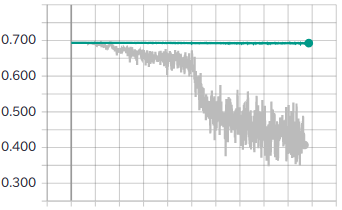
\includegraphics[width=0.5\linewidth]{img/static/max-entropy.png}
 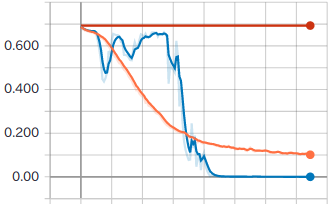
\includegraphics[width=0.49\linewidth]{img/static/val-mean-entropy.png}
 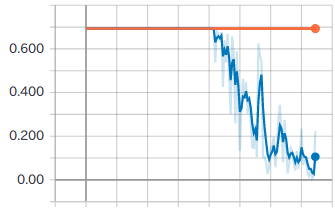
\includegraphics[width=0.49\linewidth]{img/static/val-max-entropy.png}
 \caption{
The mean (left) and the maximum (right) entropy over all bits ($N=100$) and all batch samples
while training an SAE for MNIST puzzle.
% (left: training set, right: validation set).
 % 
Compared to SAE (green), we observed that ZSAE (orange,gray,blue:$\alpha=0.2,0.5,0.7$ resp.) converges to
almost zero entropy ($\leq 10^{-2}$) around epoch 500, meaning that it finds a completely
stabilized set of symbols.
% 
% Entropy of the representation is $\sum_{i\in\{0,1\},1\leq j \leq N} -p_{ij}\log p_{ij}$ where
% $p_{ij}$, a probability that $z_{ij}=1$, is computed as $\text{Softmax}_j(\log \pi_{ij})$,
% the softmax of the un-normalized logit $\log \pi_{ij}$ used in GS.
 }
\label{ZSAE-entropy}
\end{figure}
